\documentclass{standalone}
\usepackage{tikz}
\begin{document}

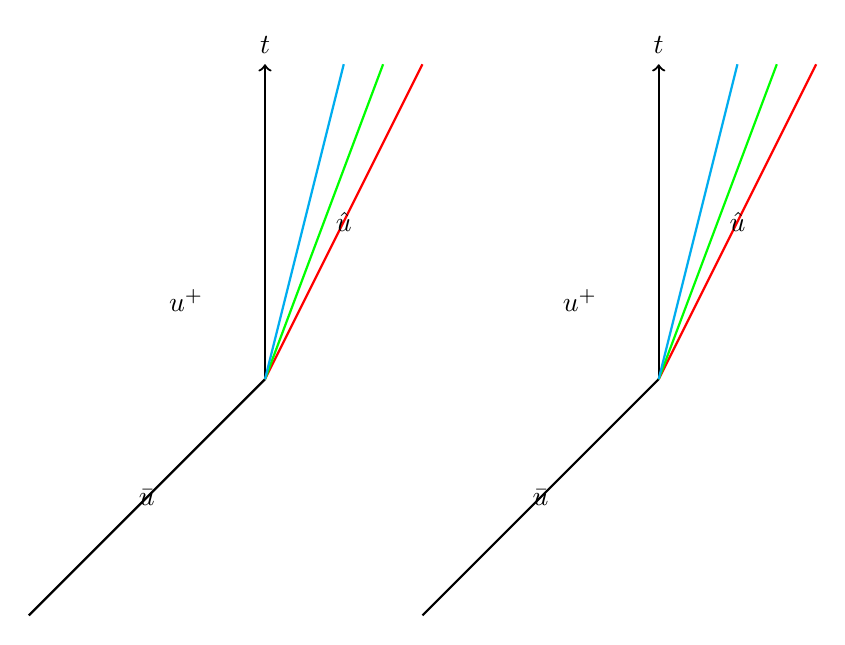
\begin{tikzpicture}

% Left diagram
\begin{scope}
    % Axes
    \draw[thick,->] (0,0) -- (0,4) node[above] {$t$};
    \draw[thick] (0,0) -- (-3,-3);

    % Wave fronts
    \draw[thick,red] (0,0) -- (2,4);
    \draw[thick,green] (0,0) -- (1.5,4);
    \draw[thick,cyan] (0,0) -- (1,4);

    % Labels
    \node at (-1.5,-1.5) {$\bar{u}$};
    \node at (1,2) {$\hat{u}$};
    \node at (-1,1) {$u^+$};
\end{scope}

% Right diagram
\begin{scope}[xshift=5cm]
    % Axes
    \draw[thick,->] (0,0) -- (0,4) node[above] {$t$};
    \draw[thick] (0,0) -- (-3,-3);

    % Wave fronts
    \draw[thick,red] (0,0) -- (2,4);
    \draw[thick,green] (0,0) -- (1.5,4);
    \draw[thick,cyan] (0,0) -- (1,4);

    % Labels
    \node at (-1.5,-1.5) {$\bar{u}$};
    \node at (1,2) {$\hat{u}$};
    \node at (-1,1) {$u^+$};
\end{scope}

\end{tikzpicture}

\end{document}